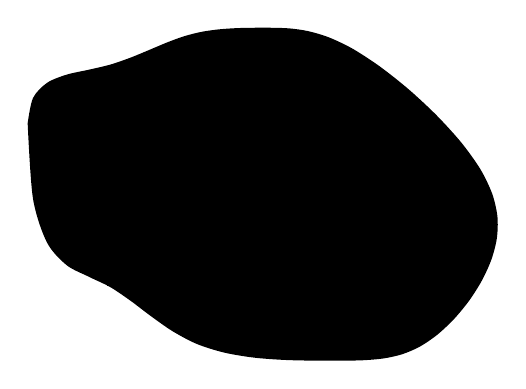
\begin{tikzpicture}[yscale=.6]%[width=\marginparwidth+25pt]
%\begin{axis}[width=\marginparwidth+25pt,%
%tick label style={font=\scriptsize},axis y line=middle,axis x line=middle,name=myplot,axis on top,%
%			%x=.37\marginparwidth,
%			%y=.37\marginparwidth,
%			xtick={1,2,3,4,5,6,7,8,9,10,11,12},% 
%%			extra x ticks={12.57},
%%			extra x tick labels={$4\pi$},
%%			ytick=\empty,
%			%minor y tick num=1,%extra y ticks={-5,-3,...,7},%
%%			minor x tick num=4,
%			ymin=-.1,ymax=8.5,%
%			xmin=-.1,xmax=12.5%
%]

\draw [{\colorone},thick,fill={\coloronefill},smooth] plot coordinates {(0,2.)(0.06639,2.527)(0.2407,2.839)(0.4857,3.009)(0.7641,3.112)(1.039,
3.221)(1.294,3.367)(1.532,3.53)(1.759,3.689)(1.98,3.823)(2.2,3.915)(2.
42,3.967)(2.64,3.992)(2.86,4.)(3.08,4.)(3.305,3.987)(3.543,3.93)(3.
808,3.797)(4.107,3.558)(4.45,3.185)(4.815,2.703)(5.17,2.152)(5.483,1.
577)(5.723,1.018)(5.872,0.5022)(5.938,0.02083)(5.93,-0.4363)(5.861,-0.
88)(5.741,-1.319)(5.58,-1.742)(5.389,-2.128)(5.179,-2.456)(4.96,-2.
705)(4.737,-2.865)(4.502,-2.953)(4.243,-2.991)(3.95,-3.)(3.614,-2.999)
(3.244,-2.984)(2.86,-2.935)(2.484,-2.829)(2.137,-2.646)(1.832,-2.378)(
1.558,-2.06)(1.299,-1.734)(1.039,-1.443)(0.7641,-1.222)(0.4857,-0.
9779)(0.2407,-0.5015)(0.06639,0.4201)(0,2.)};

\draw (1,3.22) -- (1,-1.443) node [shift={(-3pt,0pt)},rotate=90,pos=.5] {\scriptsize 4.7};

\draw (2,3.823) -- (2,-2.5) node [shift={(-3pt,0pt)},rotate=90,pos=.5] {\scriptsize 6.3};

\draw (3,4) -- (3,-2.95) node [shift={(-3pt,0pt)},rotate=90,pos=.5] {\scriptsize 6.9};

\draw (4,3.62) -- (4,-3) node [shift={(-3pt,0pt)},rotate=90,pos=.5] {\scriptsize 6.6};

\draw (5,2.4) -- (5,-2.7) node [shift={(-3pt,0pt)},rotate=90,pos=.5] {\scriptsize 5.1};

%\end{axis}
%
%\node [right] at (myplot.right of origin) {\scriptsize $x$};
%\node [above] at (myplot.above origin) {\scriptsize $y$};
\end{tikzpicture}


